\documentclass[11pt]{article}

% Page layout
\usepackage[margin=1in]{geometry}

% Spacing
\usepackage{setspace}
\onehalfspacing

% Encoding and fonts
\usepackage[utf8]{inputenc}
\usepackage[T1]{fontenc}

% Packages
\usepackage{graphicx}
\usepackage{tabularx}
\usepackage{threeparttable}
\usepackage{multirow}
\usepackage{url}
\usepackage{hyperref}
\usepackage{float}
\usepackage{natbib}
\usepackage{authblk}
\usepackage{booktabs}

\title{Nobel Prize}

\author[1,2,3,*]{Chad M.\ Topaz}
\author[2]{Arden Fleuhr}
\author[1,4]{Jude Higdon}
\author[2]{Anvi Kurongonayini}
\author[5]{Ariana Mendible}
\author[2]{Bennett Ptak}
\author[6]{Rachel Roca}
\author[3]{Nancy Rodr\'{i}guez}
\author[2]{R\'{e}gan Schwartz}
\author[7]{Lu Xian}

\affil[1]{QSIDE Institute}
\affil[2]{Williams College}
\affil[3]{University of Colorado--Boulder}
\affil[4]{Bennington College}
\affil[5]{Seattle University}
\affil[6]{Michigan State University}
\affil[7]{University of Michigan}
\affil[*]{Corresponding author: chad.topaz@gmail.com}

\begin{document}

\maketitle

\begin{abstract}
We did a project.
\end{abstract}

\section{Introduction}
\label{sec:introduction}

Within the academic community, few awards compare in professional and public prestige to the Nobel Prize. Alfred Nobel was a 19th-century scientist and inventor who amassed a fortune from the invention of dynamite and the manufacturing of armaments. Perhaps prompted by his labeling in the press as ``the merchant of death'' \citep{Gol2000}, he endowed the eponymous prizes, meant to honor ``those who, during the preceding year, have conferred the greatest benefit to mankind'' in the areas of chemistry, physics, physiology or medicine, literature, and peace \citep{NobelPrizeWebsiteFull}.

The first Nobel Prizes were awarded in 1901, and as of 2020, there were 962 winners, or \emph{laureates}. The vast majority of these are men \citep{LunJenJau2019} and most express geographic origin in Europe or North America \citep{Fis2013}. More generally, a substantial body of research identifying the overrepresentation of individuals who are white, men, cisgender, heterosexual, and/or nondisabled has brought into stark relief the degree to which minoritized individuals in certain fields must fight against exclusion in order to participate \citep{TopSen2016, TopKliBer2019, LarTay2020, ACTReport, TopHigEpp2022}. Why might this matter?

Lack of diversity and inclusion through the vertical tiers of an academic or professional field is problematic for several reasons. Diverse representation can help ensure that a professional culture and the products that emerge from it will be designed not only to avoid harm to marginalized individuals but to serve as a corrective factor for historic inequity \citep{ACTReport,WilMilKas2021}. Additionally, when individuals from marginalized groups see people who share their identity characteristics occupying high-status positions, it bolsters their ability to imagine themselves in such positions and work towards ambitious goals \citep{OysBybTer2006, WilMilKas2021}.

Geographic bias in scientific recognition deserves particular scrutiny because it compounds through a mechanism that \citet{Mer1968} termed the ``Matthew effect'': eminent scientists receive disproportionate credit, which attracts further resources and talent, which produces further eminence. When recognition systems such as the Nobel Prize preferentially channel prestige toward scientists from a few dominant regions, the resulting concentration of funding, talent, and attention reinforces itself across generations. \citet{vonZed2025} document a version of this pattern, finding that over 80\% of Nobel Prize--winning discoveries were made in just five countries. Recently, \citet{DumTep2025} showed that geographic homophily pervades peer review itself: same-country reviewers are approximately five percentage points more likely to recommend acceptance, creating what they call ``geographical representation bias'' --- a structural advantage for researchers from countries that are overrepresented among reviewers. Their finding demonstrates that geographic sorting in scientific evaluation is not limited to a single institution; it is a systemic feature of how science distributes recognition. The Nobel Prize, as the apex of that system, is a natural site at which to ask where, precisely, geographic sorting enters.

\subsection{Previous Work}

An existing body of work has examined Nobel Laureates and their demographics. For example, \citet{BafVam2011} investigate the ages of laureates and \citet{ChaEllRah2011} delve into gender, demonstrating that women laureates are less likely to marry or have children as compared to men. Perhaps unsurprisingly, laureates are overwhelmingly white, male, and affiliated with a university \citep{Cra2001}. Furthermore, many nominees come from only a few countries; for example, between 1901 to 1951, three-quarters of physics nominees came from the US, Britain, Germany, and France, while none came from the continent of Africa \citep{Cra2001}. Laureates enjoy a range of benefits such as more citations of their work, more freedom to focus on their work, increased funding, and global publicity \citep{CasFan2013}. Indeed, \citet{WagHorWhe2015} find that laureates produce fewer papers than matched peers but with higher average citations, and that laureates occupy more central positions in coauthorship networks, suggesting that recognition and network centrality reinforce one another.

Arguably, identifying who has \textit{not} won a Nobel Prize is a richer line of questioning and one that has been around since the prize's conception. In terms of gender biases, the lack of women in STEM fields does not account fully for the low number of female laureates; with strong confidence, women are under-represented \citep{LunJenJau2019}. \citet{ModGilSha2018} trace the long-standing gendered barriers in scientific recognition, documenting how women scientists have historically been excluded from nomination despite demonstrable contributions. The very conditions needed for Nobel Prizes have also excluded and created conflict from its conception. For example, the rule that only three individuals can share a prize for a given advancement erases invaluable work done in collaboration with more scholars. The exclusion of certain collaborators has caused several controversies throughout the years, as listed by \citet{CasFan2013} and \citet{Led2016}. Only living scientists may be awarded a Nobel Prize, which puts the onus on recognizing individuals for their contribution before they are disqualified by death. Several collaborators did not share Nobel Prizes for their contributions for this very reason \citep{CasFan2013}. Beyond gender, \citet{NeiVueVue2024} examine racial and national disparities among laureates in physiology or medicine, finding stark underrepresentation of Black scientists and highlighting persistent gaps in data reporting on ethnicity, gender identity, and disability that limit intersectional analysis.

Nobel prizes are awarded to those ``conferred the greatest benefit on mankind'' \citep{nobelwill}, but choosing who has made the most important contribution is a subjective and inevitably biased choice that depends heavily on those with direct participation in the process. Preferences for theoretical or experimental work, lack of broad international support, grudges, and previous awards in similar areas of study all affect who wins the award \citep{But2016, Cra2001, CasFan2013}. But the committee is not the only way bias can enter the Nobel system. \citet{BafVam2011} highlight this nuance by writing ``if there is a preference for older Nobel candidates, this is introduced during the nomination process.'' \citet{GalDom2019} use network analysis to show that nominations are shaped by homophily, with nominators tending to favor individuals from similar national and institutional backgrounds, and that nominees endorsed by central, prestigious actors are more likely to become laureates. \citet{KoJanYan2024} further demonstrate that national favoritism, or ``particularism,'' pervades the nomination process, with wealthy nations disproportionately nominating their own citizens and political, economic, and colonial factors influencing recommendations independently of scientific merit. Despite mounting evidence of these biases, a recent Nature editorial observed that progress toward diversity in science prizes remains slow and called for greater transparency in nomination data \citep{Nature2022}.

Yet a fundamental question remains unanswered: at which stage of the Nobel Prize's multi-step selection pipeline does geographic sorting enter? The question matters because the answer determines where reform can be effective. \citet{GalDom2019} built a nominator--nominee network for the Physics prize, demonstrating that homophily exists, but their single-layer, single-discipline design could not distinguish institutional sources of bias from individual ones, nor determine whether the pattern generalizes across prizes. \citet{KoJanYan2024} quantified national favoritism across the sciences using regression, but treated the nomination system as a single stage and could not decompose the institutional hierarchy that connects governing bodies, vetting committees, nominators, nominees, and laureates. Answering the ``where'' question requires an analytical framework that represents each institutional layer and each type of decision as a separate edge in a multilayer network --- a structure that, to our knowledge, has not previously been constructed for any scientific prize system.

\subsection{Nobel Prize Selection Process}

Nobel Prize selection processes are complex and opaque. One reason for the lack of clarity is that there appears to be no definitive scholarly source, and indeed no single source at all, with a complete description of these processes. We now aim to fill this surprising gap in the literature. The discussion that follows draws from online sources, namely the websites of the \citet{NobelPrizeWebsiteFull}, the \citet{RSAS}, the \citet{KINA}, and the Wikipedia entry for the Nobel Peace Prize \citep{NPPWiki}.

Table~\ref{Tab1} summarizes relevant actors for the selection of the five Nobel Prizes. Here, we focus on the individuals who wield influence on the process, and so we do not include nominees and laureates in the table. We begin with a general discussion of the various actors and, subsequently, proceed to a more detailed discussion for each specific Nobel Prize.

\newcolumntype{s}{>{\raggedright\arraybackslash} p{0.15\textwidth}}
\begin{table}[t!]
\footnotesize
\begin{threeparttable}
\caption{Overview of the process for selection of Nobel Laureates. For each Nobel Prize, a governing body chooses from among a group of potential vetters in order to create a vetting body. The vetting body receives nominations made by nominators and creates a short list of viable laureates. The selection body takes the vetting body's input and makes the final choice of laureate.\label{Tab1}}
\bigskip
\begin{tabular}{p{0.12\textwidth}sssss}
               & \bf Chemistry                                          & \bf Physics                                            & \bf Physio/Med                             & \bf Literature                           & \bf Peace                                                      \\ \cline{2-6}
               &&&&& \\
\bf Governing Body & Royal Swedish Academy of Sciences                  & Royal Swedish Academy of Sciences                  & Nobel Assembly at Karolinska Institutet               & Swedish Academy                      & Storting\tnote{1}                                                   \\
&&&&&\\
\bf Potential Vetters    & Royal Swedish Academy of Sciences                  & Royal Swedish Academy of Sciences                  & Karolinska Institutet                                & Swedish Academy                      & Norwegian politicians\tnote{2} \\
&&&&&\\
\bf Vetting Body   & Nobel Committee for Chemistry\tnote{3}                      & Nobel Committee for Physics\tnote{3}                        & Nobel Committee for Physio/Med                & Nobel Committee for Literature\tnote{3}       & Norwegian Nobel Committee                                  \\
&&&&&\\
\bf Nominators     & By invitation based on stated eligibility criteria & By invitation based on stated eligibility criteria & By invitation based on stated eligibility criteria & Based on stated eligibility criteria\tnote{4} & Based on stated eligibility criteria                       \\
&&&&&\\
\bf Selection Body & Royal Swedish Academy of Sciences                  & Royal Swedish Academy of Sciences                  & Nobel Assembly at Karolinska Institutet                & Swedish Academy                      & Norwegian Nobel Committee \\ \\ \cline{2-6}
\end{tabular}
\bigskip
\begin{tablenotes}
\item[1] The Storting is the Norwegian parliament.
\item[2] It is not a formal eligibility requirement to be a politician, nor to be Norwegian. However, the Storting has stated that ``As far as possible, the composition of the Committee is to reflect the relative strengths of the political parties in the Storting.'' Moreover, historically, all members of the committee have indeed been Norwegian.
\item[3] Five members of the Vetting Body are chosen by the Governing Body, and then several additional members of the Vetting Body are added by the Vetting Body itself; these are called \emph{co-opted} members.
\item[4] Similar to the Vetting Bodies for Chemistry, Physics, and Physiology/Medicine, the Vetting Body for Literature does send out letters soliciting nominations. However, unlike for those other prizes, for the Literature prize, individuals who meet certain eligibility requirements can nominate even if they did not receive a letter of invitation to do so.
\end{tablenotes}
\end{threeparttable}
\end{table}

Each prize has a \emph{governing body} that oversees the nomination and selection processes. This governing body chooses from among \emph{potential vetters} to create a \emph{vetting body}. The vetting body is in charge of soliciting and/or receiving nominations. \emph{Nominators} are the individuals who nominate candidates for the different awards.  For three of the five awards, individuals who meet certain criteria can become nominators only by invitation of the vetting body. For the other two awards, \emph{any} individual who meets the stated criteria for eligibility can nominate. After receiving nominations, the vetting body sends out nominee portfolios to experts (who do not appear in the table) for evaluation, assesses the nominees, and suggests a shortlist of possible laureates to the governing body. This \emph{governing body} makes the final selection of laureate(s).

Each specific Nobel Prize selection process has unique nuances. The prizes with the most similar processes are the Nobel Prizes in Chemistry and Physics. The governing body for both awards is the Royal Swedish Academy of Sciences (RSAS), established in 1739 as an independent organization to promote the influence of science across the globe. New members are elected by current members. Today, the RSAS has about 480 Swedish and 175 foreign members, divided by discipline into ten classes. The Nobel Committees for Chemistry and Physics are the vetting bodies, respectively, for the prizes. Each committee is made up of five voting members from the relevant RSAS class. The first task of the vetting body is to send out forms to qualified individuals asking for nominations. Typically, each committee receives 250 - 300 nominations. Eventually, based on externally solicited evaluations and its own deliberations, each committee prepares a report with a list of finalists. During the final selection meeting of the RSAS, all present members of the RSAS discuss the report and vote on a finalists. One to three candidates are selected each year for each prize.

The Nobel Prize in Physiology and Medicine involves different actors. The governing body is the Nobel Assembly at the Karolinska Institutet, which is a medical research institute in Sweden. Since 1984, the Nobel Assembly is composed of 50 members of that institute. The vetting body is the Nobel Committee for Physiology or Medicine and consists of five voting members appointed by the Nobel Assembly from among the Karolinska Institute. The selection body, which chooses the laureate(s), is the Nobel Assembly.

The Nobel Prize in Literature is governed by the Swedish Academy (not to be confused with the RSAS). The Swedish Academy is composed of 18 members who are appointed for life.  The Nobel Committee for Literature, the vetting body, is selected from among the members of the Academy for a three-year term.  While the vetting body sends letters to qualified individuals to solicit nominations, \emph{anyone} who is qualified, as stated by prescribed eligibility criteria, may nominate a candidate. The laureate is selected by the Swedish Academy from among a list of finalists proposed by the Nobel Committee.

Finally, for the Nobel Peace Prize, the \emph{Storting}, or the Norwegian parliament, is the governing body.  The Storting elects members of the Norwegian Nobel Committee, the vetting body, for six-year terms (with potential for re-election).  Unlike the previous prizes discussed, the Norwegian Nobel Committee does not solicit nominations from qualified nominators. Rather, anyone who meets the stated eligibility criteria can nominate. Also, in contrast to the other prizes, the selection body for the Nobel Peace Prize is \emph{not} the same as the governing body. Rather, it is the Norwegian Nobel Committee, which also serves as the vetting body.

The present study addresses the ``where'' question directly. We construct the first multilayer network of the Nobel Prize selection process, spanning all five original prize categories from 1901 through the most recent year of publicly available nomination data. The network encompasses five institutional layers --- governing bodies, vetting bodies, nominators, nominees, and laureates --- assembled from over a dozen sources into a reproducible pipeline. Unlike prior single-layer or regression-based approaches, this structure allows us to decompose geographic homophily by edge type, isolating the specific decision point at which geographic sorting enters an otherwise neutral institutional process.

Our primary results are threefold. First, geographic homophily is concentrated almost entirely in the nominator $\to$ nominee edge; the institutional edges connecting governing bodies, vetting bodies, and laureates show negligible homophily. This is a result that prior work could not obtain: without decomposing the network by edge type, there was no way to know whether the Swedish-led institutions or the individual nominators were responsible for the geographic sorting that earlier studies had detected only in aggregate. Second, this homophily varies across prizes in a pattern consistent with the internationality of each discipline's knowledge networks, from Literature (highest) to Physics (lowest). Third, the homophily ratio has increased over time even as the nominee pool has diversified, revealing a paradox in which the system has become more globally inclusive in absolute terms while becoming more geographically biased in relative terms. Together, these findings identify the nomination stage as the critical intervention point for any effort to reduce geographic bias in the world's most prestigious recognition system.

\section{Methods}
\label{sec:methods}

\subsection{Network Model}
\label{sec:networkmodel}

Given the many different actors involved in Nobel Prize selection, and given the ambient hierarchical structure, we adopt a multilayer network modeling framework. In the most fundamental network models, there are nodes that are potentially connected by edges, and there is a single type of each. In other words, the nodes describe a single set of entities and the edges represent a single type of relationship between them. However, some modeling situations might instead suggest the use of multiple types of nodes and different levels of connections. These networks are called multilayer networks. See \citet{KivAreBar2014} for a comprehensive introduction, including many applications and examples.

To begin proposing a network model, we revisit Table~\ref{Tab1}. As previously described, this table outlines five different categories of actors who potentially influence the final choice of Nobel Laureates. We have two simplifications. First, in our model, we will ignore potential vetters. While potential vetters can be described for some of the prizes, it is not practical to tabulate the set of all Norwegian politicians, which would be necessary for the Nobel Peace Prize. Moreover, for the other four prizes, the potential vetters are either identical to or a superset of the governing body. The second simplification comes from the observation that the selection body is identical to a body at a higher stage of the hierarchy. For the chemistry, physics, physiology/medicine, and literature prizes, the selection body is the same as the governing body. For the Nobel Peace Prize, the selection body is the same as the vetting body. Therefore, we do not include the selection body in our model.

In summary of what we have outlined thus far, we will include in our model three of the bodies in Table~\ref{Tab1}, namely the governing body, the vetting body, and the nominators. In addition, we will include two groups who represent the eventual result of decisions made by the three aforementioned bodies, namely, nominees and laureates. Thus, our model will describe the governing body, the vetting body, nominators, nominees, and laureates for each of the Nobel Prizes. We will place these in a five-layer network with the governing body at the top and the laureates at the bottom. Fig.~\ref{Fig1} provides a schematic view.

\begin{figure*}[t!]
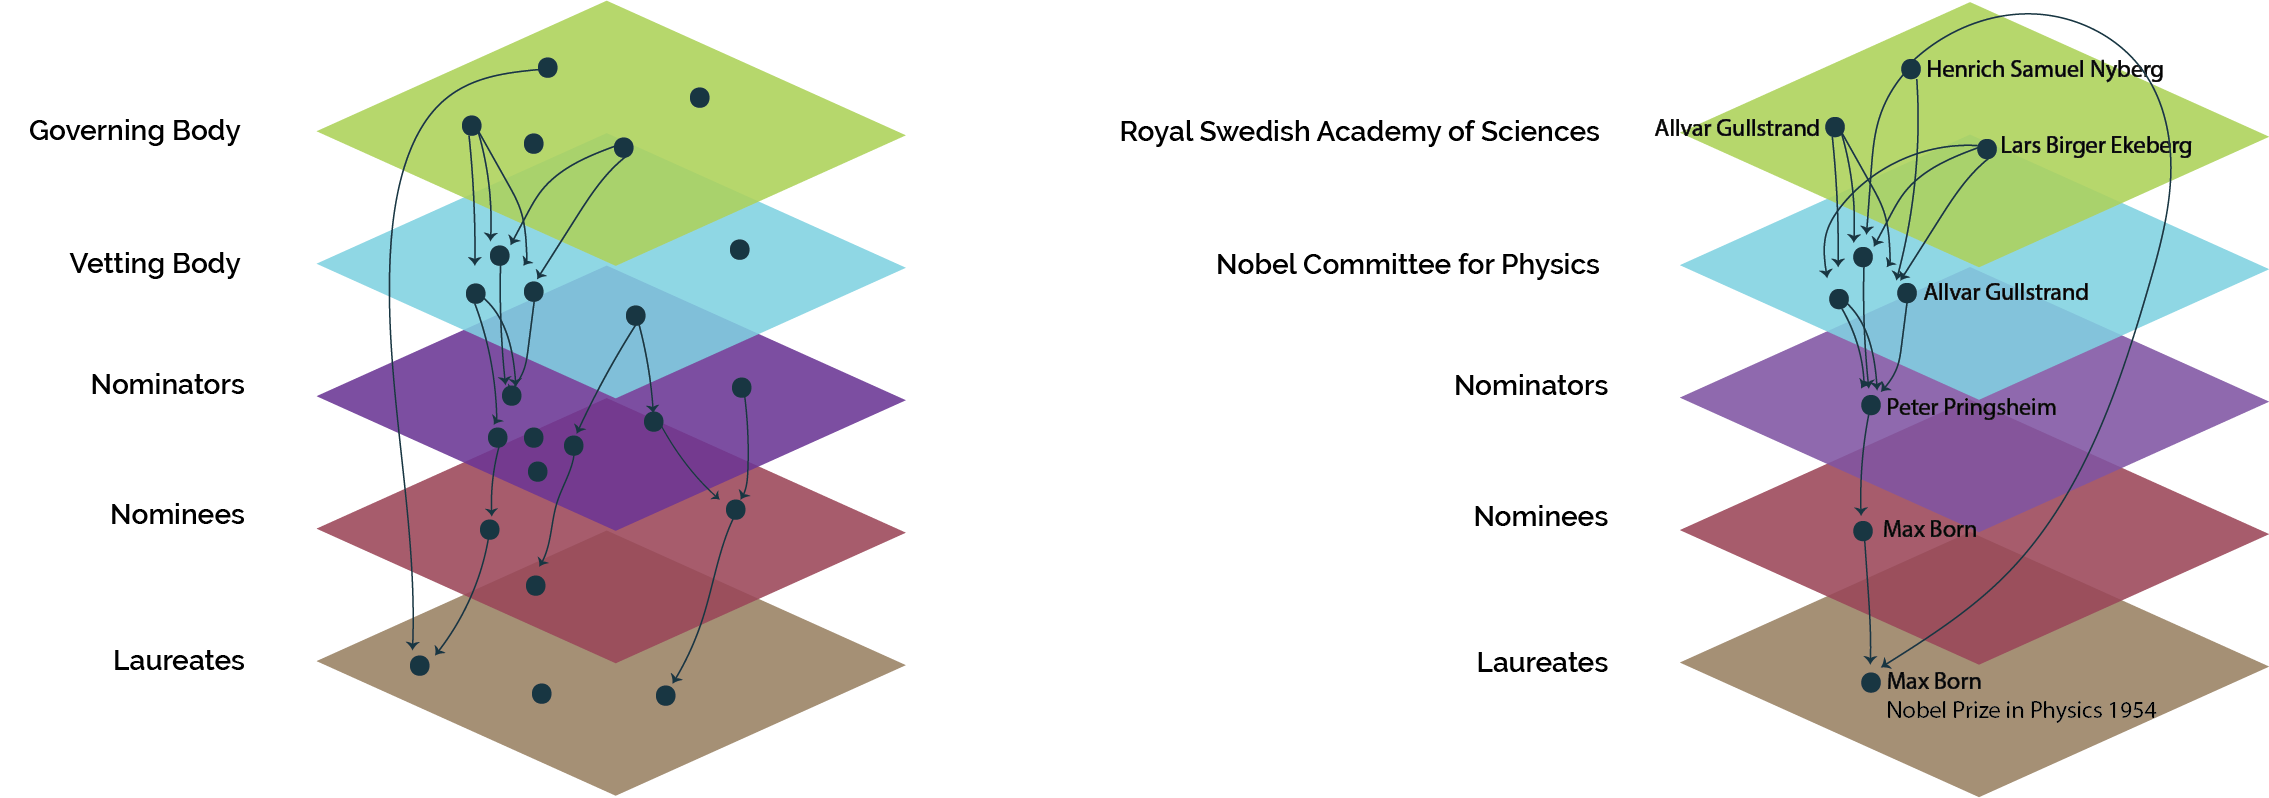
\includegraphics[width=\textwidth]{Fig1.png}
\caption{Multilayer network modeling framework for Nobel Prize selection. These are minimal schematic diagrams that include only a small subset of nodes and a small subset of the edges that actually exist between those nodes. More complete visualizations appear in Sec.~\ref{sec:results}. Left: Schematic of the five layers of our network as described in Sec.~\ref{sec:networkmodel}, namely, governing body, vetting body, nominators, nominees, and laureates. Nodes represent individuals and directed edges indicate decision-making power. That is to say, an edge pointing from person A to person B indicates that A was one of the people responsible for selecting B. The schematic at right is a (partial) example of the Nobel Prize in Physics from 1958. For the physics prize, the governing body is the Royal Swedish Academy of Sciences and the vetting body is the Nobel Committee for Physics; see Table~\ref{Tab1}.\label{Fig1}}
\end{figure*}

In constructing the prize selection network, we must keep in mind the various complexities of data. For instance, trivially, any laureate must also appear as a nominee. But beyond that, individuals may serve in multiple other roles, potentially in different years and for different prizes. For example:
\begin{itemize}
\item Willem Einthoven won the Nobel Prize in Physiology or Medicine in 1924 and nominated others for that same prize in 1901, 1905, 1917, and 1921.
\item Marie Curie was nominated for the Nobel Prize in Physics in 1902 and 1903, winning it in the latter year. She nominated other individuals for this prize in 1905 and 1910. Additionally, she was nominated for the Nobel Prize in Chemistry in 1911 and won it.
\item Bj{\o}rnstjerne Bj{\o}rnson was one of the original members of the Nobel Peace Prize vetting/selection body, the Norwegian Nobel Committee, from 1901 through 1906. He nominated other individuals for that prize in 1902, 1903, and 1907.  He himself was nominated for the Nobel Prize in Literature in 1902 and 1903, winning it during the second year.
\end{itemize}

To capture complexities like the aforementioned ones, we keep track of our data in the following manner. We represent each unique individual as a node. We attach to that node any personal demographics that are not directly tied to prize selection, such as gender, nationality, and so forth. Then, we apply edges to capture the roles of these individuals across prizes and across time. More specifically, each edge carries with it not just the specification of two nodes, but also a year, a Nobel Prize, and two network layers. For example, take the case of Marie Curie above. One of Curie's nominators for the Chemistry Prize in 1911 was Gaston Darboux. Therefore, our network has a directed edge pointing from Darboux to Curie. That edge specifies the year 1911, the field of chemistry, and the two network layers of nominators and nominees. Since Curie nominated Joseph Thomson for the Nobel Prize in Physics in 1905, the network has an edge pointing from Curie to Thomson. That edge specifies the year 1905, the field of physics, and, again, the two network layers of nominators and nominees.

\subsection{Data Acquisition}
\label{sec:dataacquisition}

There is no single source from which one can obtain all of the data necessary to construct the network model. We gather the necessary data for the five layers from a variety of sources, summarized in Table~\ref{tab2}. While information about governing bodies, vetting bodies, and laureates is available up through the present day, information about nominators and their nominees is made public only 50 years after the fact, subject to a secrecy rule imposed by the Nobel Foundation. All data gathering was performed programmatically in R using a reproducible pipeline of nine scripts, available in a public repository \citep{nobelgithub}. Below we describe each stage in sufficient detail for independent replication.

There are two broad steps to assembling the data. First, we must determine the identities of the individuals in each network layer and when they served. Then we must determine the relevant characteristics of those individuals, such as personal demographics. For the first step, we use the sources listed in the final column of Table~\ref{tab2}. For the second step, we use Wikidata \citep{wikidata}, a structured open knowledge database that, among other roles, provides the structured data behind many Wikipedia pages. By using Wikidata as our source for individual characteristics, we implicitly adopt the choices made by its contributors. As merely one example, we ourselves do not weigh in with inferences of individuals' gender; we use the gender data vetted by Wikidata, recognizing that any demographic data that is not self-identified is imperfect. Throughout the pipeline, we use Wikidata QIDs (unique entity identifiers of the form Q followed by a number) as the canonical identifier for each individual, enabling cross-referencing across data sources.

\begin{table}[t!]
\begin{tabular}{lll}
\textbf{Network Layer(s)}     & \textbf{Body}                       & \textbf{Source}                                                                                                                                    \\ \hline
                              &                                     &                                                                                                                                                    \\
Governing Body/Selection Body & Royal Swedish Academy of Sciences   &  \citet{Ledamotsregister}   \\
                              & Karolinska Institutet               &   \citet{KarolinskaEmployees}             \\
                              & Swedish Academy                     &  \citet{Ledamotsregister}                 \\
                              & Storting                            & \citet{wikidata}                          \\
                              &                                     &                                                                                                                                                    \\
Vetting Body                  & Nobel Committee for Chemistry       & \citet{NobelCommitteeChemistry}  \\
                              & Nobel Committee for Physics         &  \citet{NobelCommitteePhysics}   \\
                              & Nobel Committee for Physio/Med &  \citet{NobelCommitteePhysiology}             \\
                              & Nobel Committee for Literature      &   \citet{Ledamotsregister}              \\
                              & Norwegian Nobel Committee           &  \citet{NorwegianNobelCommittee}                  \\
                              &                                     &                                                                                                                                                    \\
Nominators                    &                                     & \citet{NobelPrizeWebsite}                                                  \\
                              &                                     &                                                                                                                                                    \\
Nominees                      &                                     & \citet{NobelPrizeWebsite}                                               \\
                              &                                     &                                                                                                                                                    \\
Laureates                     &                                     & Nobel Prize API v2.1                                                                                                                                           \\ \hline
\end{tabular}
\caption{Sources for the data in each network layer.\label{tab2}}
\end{table}

\subsubsection{Governing Bodies}
\label{sec:data-governing}

\textbf{Royal Swedish Academy of Sciences (RSAS).} The RSAS awards the prizes in Physics and Chemistry. Members are elected for life; their service begins at induction and ends at death. We scraped the membership list from the Swedish-language Wikipedia page \emph{Lista \"over ledam\"oter av Kungliga Vetenskapsakademien} \citep{Ledamotsregister}, which organizes members chronologically under bold year headers followed by bulleted lists of hyperlinked member names. Founding members (1739) appear under the headings ``Akademiens grundare'' and ``\"Ovriga.'' We parsed the rendered HTML by iterating through child elements in document order, updating the current induction year whenever a bold year header was encountered, and extracting all hyperlinked names from subsequent unordered lists. We excluded redlinks (articles not yet created) and non-article links.

Wikidata QIDs were resolved in batch using the MediaWiki \texttt{action=query\&prop=pageprops} API, which maps up to 50 Wikipedia page titles to their corresponding Wikidata items per request. This API also handles title normalization (e.g., converting underscores to spaces and resolving Unicode variants), which we accounted for when matching responses to input titles. We used exponential backoff (delay doubling from 2 seconds, up to 5 retries) for failed requests and imposed a 0.2-second delay between batches. For each member, we recorded the induction year as the start year; end years were left initially blank and later imputed from Wikidata death dates (see Section~\ref{sec:data-demographics}). Where multiple records existed for the same QID (e.g., due to class transfers within the Academy), we retained only the earliest induction record. The final dataset contains 2{,}312 RSAS members spanning 1739--2025, all with resolved QIDs.

\textbf{Swedish Academy.} The Swedish Academy awards the Prize in Literature. Its 18 members are appointed for life. We queried Wikidata directly via SPARQL, selecting all individuals holding position (P39) ``member of the Swedish Academy'' (Q207360), excluding honorary members (Q97563901). Start and end dates were extracted from the \texttt{pq:P580} and \texttt{pq:P582} qualifiers on each position statement and parsed from Wikidata's ISO~8601 datetime format (e.g., \texttt{1871-12-20T00:00:00Z} $\to$ 1871). All SPARQL queries throughout the pipeline were executed via HTTP POST to the Wikidata Query Service endpoint, with results returned in JSON format. We implemented retry logic with exponential backoff (5-second base delay, up to 10 retries) and identified our bot with a descriptive User-Agent string per Wikidata's access policy. The query yielded 202 member records.

\textbf{Storting (Norwegian Parliament).} The Storting awards the Peace Prize. We queried Wikidata for all entities classified as human (P31 = Q5) holding position (P39) ``member of the Storting'' (Q9045502), extracting start and end dates from position qualifiers. Norwegian parliamentarians may serve non-consecutive terms; we consolidated consecutive terms by grouping each member's service periods chronologically and merging periods where the gap between one term's end year and the next term's start year was at most one year. Non-consecutive terms were preserved as separate records. This yielded 4{,}281 member-term records spanning 1814--2025.

\textbf{Karolinska Institutet.} The Karolinska Institutet (KI) awards the Prize in Physiology or Medicine. Prior to 1977, all full professors at KI constituted the selection body; in 1977 the Nobel Assembly was established as a distinct entity, and in 1984 its membership was fixed at 50. Neither Wikidata nor KI's website publishes a complete roster of the Nobel Assembly.

We compiled KI professor data from Project Runeberg's digitized editions of the Swedish state calendar (\emph{statskalendern}) \citep{KarolinskaEmployees}, covering 1881--1970. Fourteen editions were manually mined for each professor's name, start year, and end year. Separately, Wikidata QIDs were searched and connected to each individual, verifying that biographical information matched or was plausible. The resulting spreadsheet contains one row per professor; we retained the 140 records with confirmed QIDs and both start and end years.

Post-1970 Nobel Assembly membership is not publicly available: Wikidata contains essentially no position (P39) or membership (P463) records for the Nobel Assembly entity (Q3375124), KI's website does not publish a member roster, and Project Runeberg's digitized calendars stop circa 1972. This is a known structural gap in our data (see Section~\ref{sec:gaps}).

\subsubsection{Vetting Bodies (Nobel Committees)}
\label{sec:data-vetting}

Each prize has a dedicated Nobel Committee that reviews nominations and prepares recommendations for the governing body.

\textbf{Chemistry, Physics, and Physiology/Medicine Committees.} These three committees are documented on Swedish-language Wikipedia \citep{NobelCommitteeChemistry,NobelCommitteePhysics,NobelCommitteePhysiology}. We extracted membership lists using a general-purpose parser that fetches wikitext (not rendered HTML) via the MediaWiki API (\texttt{action=parse\&prop=wikitext}), splits the text into sections by heading markers, and extracts bullet-list entries from sections titled ``Tidigare ledam\"oter'' (former members), ``Nuvarande ledam\"oter'' (current members), and ``Sekreterare'' (secretaries). Each entry follows one of several Swedish Wikipedia conventions: \texttt{[[Name]], YYYY--YYYY} (former members with date range), \texttt{[[Name]], invald YYYY} (current members, Swedish format), or \texttt{[[Name]], YYYY--} (current members, open-ended). We parsed Wikipedia article titles from double-bracket link syntax, extracted start and end years via regular expressions, and resolved QIDs through the batch MediaWiki API. The Swedish Wikipedia page for the Physiology/Medicine committee explicitly states ``Listan \"ar ofullst\"andig'' (the list is incomplete). Final counts: Chemistry 50 members, Physics 51, Physiology/Medicine 72 (59 with QIDs).

\textbf{Literature Committee.} The Nobel Committee for Literature is drawn from the Swedish Academy. No standalone membership list exists on Wikipedia. Instead, we extracted committee service years from individual member biographies on \texttt{svenskaakademien.se} \citep{Ledamotsregister}. We first queried Wikidata for all Swedish Academy members with their seat numbers (extracted from position labels matching the pattern ``member of the Swedish Academy at seat $N$''). We then constructed biography page URLs following the site's convention: \texttt{/de-aderton/stol-nr-\{seat\}-\{name-slug\}}, where the name slug is a lowercased, hyphen-separated, ASCII-transliterated version of the member's name.

The Swedish Academy website is built as a Nuxt.js single-page application. Rather than executing JavaScript, we extracted biography text directly from the \texttt{\_\_NUXT\_DATA\_\_} script tag embedded in each page's HTML source. This payload contains HTML-encoded biography text; we decoded HTML entities, stripped markup tags, and searched for mentions of ``Nobelkommitt\'en'' followed by year ranges. Two-digit years were expanded to four digits based on context (e.g., ``1969--86'' $\to$ 1969--1986). We retained only members whose biographies mentioned Nobel Committee service, yielding 35 members. This extraction method is fragile to future website redesigns.

\textbf{Norwegian Nobel Committee.} The Norwegian Nobel Committee both vets nominations and awards the Peace Prize. We parsed the membership table from the English Wikipedia page \emph{List of members of the Norwegian Nobel Committee} \citep{NorwegianNobelCommittee}, extracting start and end years and resolving QIDs via the batch MediaWiki API. This yielded 61 members (57 with QIDs).

\subsubsection{Nominations}
\label{sec:data-nominations}

We scraped the Nobel Prize Nomination Archive \citep{NobelPrizeWebsite}, which is subject to a 50-year secrecy rule. As of 2025, nomination records are available through 1974 or 1975 for Physics, Chemistry, Literature, and Peace. Physiology or Medicine nominations are available only through 1953; the Karolinska Institutet has not released records for 1954--1974, likely related to the 1977 Swedish transparency law and the concurrent restructuring that created the Nobel Assembly.

The archive's web interface uses numeric prize codes in its URL parameters: Physics = 1, Chemistry = 2, Physiology or Medicine = 3, Literature = 4, Peace = 5. For each of 353 prize-year combinations, we first retrieved the list page and extracted all nomination IDs from links to detail pages. We then scraped each detail page to extract the nomination year, prize category, the names and internal person IDs of all nominees and nominators, and per-nomination contextual fields. Detail pages use a two-column table layout with bold section headers (``Nominee:'' and ``Nominator:'') followed by labeled rows containing person links and metadata. For nominees, the available contextual fields are university, city, country, and (for some prizes) profession; for nominators, the available fields are profession, university, city, and country. We parsed each detail page by iterating through table rows in document order, tracking the active section header, and accumulating labeled fields (identified by \texttt{<span class="rubr">} tags) for each person block. Country values were cleaned by stripping trailing ISO~3166 codes (e.g., ``SWEDEN (SE)'' $\to$ ``SWEDEN''). A single nomination may list multiple nominees (16.3\% of nominations) and, more rarely, multiple nominators (1.1\%), reflecting joint nominations and co-signed nomination letters; we generated all pairwise nominee--nominator combinations.

Prize names were standardized to a common vocabulary (e.g., ``Physiology or Medicine'' $\to$ ``Physiology/Medicine''). The Peace Prize archive uses the header format ``Nomination for Nobel Peace Prize'' rather than ``Nobel Prize in \ldots'' as used by the other four categories; we handled this as a special case in parsing. List pages were fetched sequentially with 0.5-second inter-request delays; detail pages were fetched in parallel across $N-1$ CPU cores (capped at 12) with 0.2-second per-worker delays. Partial results were checkpointed to disk after each prize-year to allow resumption. The final dataset contains 27{,}958 nomination records spanning 22{,}600 unique nominations, 4{,}006 unique nominees, and 11{,}650 unique nominators. Among these, 780 records (2.8\%) have anonymous or unlisted nominators, and 2 records represent self-nominations.

\subsubsection{Laureates}
\label{sec:data-laureates}

We retrieved all Nobel Prize laureates from the official Nobel Prize API (v2.1, \texttt{api.nobelprize.org/2.1/laureates}), which provides structured JSON data including Wikidata QIDs, names, gender, award year, prize category, prize portion, motivation text, and primary affiliation at the time of award. We paginated through all results and filtered to the five original prize categories, excluding the Sveriges Riksbank Prize in Economic Sciences (established 1969). Laureates who received multiple prizes (7 individuals, including Marie Curie, Linus Pauling, Frederick Sanger, John Bardeen, and K.~Barry Sharpless) appear as separate records per prize. The final dataset contains 927 laureate-prize records representing 919 unique individuals, with 100\% QID coverage.

\subsubsection{Entity Resolution for Nomination Archive People}
\label{sec:data-entity-resolution}

The nomination archive identifies people by internal numeric IDs and names only, without Wikidata QIDs or other persistent identifiers. To integrate nomination data with the rest of the network (which uses Wikidata QIDs as the canonical identifier), we developed a two-stage matching procedure.

In the first stage, for each of the 14{,}474 unique people in the nomination archive, we scraped their detail page on \texttt{nobelprize.org}, extracting last name, first name, gender, birth year, and death year from labeled table cells. Scraping was parallelized across available cores in chunks of 500, with partial results checkpointed to disk. Of the 14{,}474 people, 4{,}571 (31.6\%) had birth years recorded; the remaining 9{,}903 (68.4\%) lacked birth year data entirely. Six records contained non-standard gender codes in the source database; we verified the identities of all six individuals by first name and confirmed they are male, recoding accordingly. One record had a transposed death year (1886 instead of 1986), which was corrected manually.

In the second stage, for each person with both a name and birth year (4{,}570 matchable individuals), we implemented a three-phase Wikidata matching procedure. In Phase~1, we generated up to three name variants for each person --- full name, first-plus-last name, and last name only --- and searched the Wikidata entity search API (\texttt{wbsearchentities}, limited to 15 candidates per variant) in parallel, collecting all candidate QIDs. In Phase~2, we deduplicated the candidate QIDs across all people and batch-fetched their birth years from Wikidata (property P569) via SPARQL in groups of 50. A match was accepted only when a candidate's Wikidata birth year exactly equaled the birth year recorded in the Nobel archive. We did not attempt fuzzy name matching or approximate year matching, prioritizing precision over recall. In Phase~3, we exploited the nondeterministic ordering of Wikidata's search API: for individuals still unmatched after Phase~2, we repeated the full-name search up to 100 additional times, as each query may surface different candidates. Birth year lookups from previous phases were cached, so only newly encountered QIDs required verification. Phase~3 terminated when no new matches were found in a pass or the maximum number of passes was reached.

This procedure matched 3{,}951 of 4{,}570 matchable individuals (86.5\%), representing 27.3\% of all nomination archive people. Among matched individuals, 44 had multiple Wikidata candidates with matching birth years; for these, we retained the API's top-ranked candidate and recorded the multi-match count for potential manual review. An additional 619 matchable individuals (4.3\%) remained unmatched despite having birth year data, likely because their Wikidata entries use different name transliterations or do not appear among the API's top search results. The remaining 9{,}904 people (68.4\%) lacked birth year data entirely, rendering Wikidata disambiguation infeasible. Unmatched and unmatchable individuals are represented in the network using temporary identifiers with a \texttt{NOM:} prefix (e.g., \texttt{NOM:7283}), preserving the nomination-layer topology even where cross-layer entity resolution was not possible.

\subsubsection{Demographic Enrichment}
\label{sec:data-demographics}

We fetched demographic attributes from Wikidata for all individuals with resolved QIDs across all data sources. The SPARQL query retrieved: English name label, gender (P21), country of birth (P19, traversed to sovereign state via P17), nationality (P27), birth date (P569), death date (P570), occupation (P106), and employer/institution (P108). Queries were executed in batches of up to 200 QIDs using the SPARQL \texttt{VALUES} clause, with individual fallback queries for any batch that failed. Multi-valued fields (nationality, occupation, institution) were collapsed into semicolon-delimited strings. Where multiple birth or death dates existed for a single QID (e.g., due to conflicting Wikidata sources), we retained the first non-missing value. After the initial demographic fetch for governing body, vetting body, and laureate QIDs, we performed a second pass to fetch demographics for the 3{,}951 matched nomination archive people, then re-collapsed all records to produce a single row per QID.

As a post-processing step, we imputed end-of-service years for RSAS members (who serve for life) using Wikidata death years. Of 2{,}312 RSAS members, 1{,}871 received imputed end years; 441 remain without end years (likely living members or individuals with unknown death dates). The final demographics table contains 10{,}206 unique individuals.

\subsubsection{Geographic Standardization}
\label{sec:data-geography}

Country names in our data originate from two distinct sources with different conventions: Wikidata English labels (mixed case, including historical entities such as ``Austrian Empire,'' ``Kingdom of Prussia,'' and ``Russian Empire'') and the Nobel Prize nomination archive (uppercase modern and legacy names, sometimes annotated with ISO codes or legacy state names). To enable geographic analysis, we standardized all country names to modern sovereign states, United Nations M49 subregions (14 values), and continents (6 values) using a comprehensive case-insensitive mapping table covering approximately 250 observed name variants across both data sources.

Historical entities were mapped to their most commonly associated modern successor state (e.g., Austrian Empire and Austria-Hungary $\to$ Austria; Kingdom of Prussia and German Empire $\to$ Germany; Russian Empire and U.S.S.R.\ $\to$ Russia; Czechoslovakia $\to$ Czech Republic; Ceylon $\to$ Sri Lanka). Nomination archive country fields were pre-cleaned by stripping legacy annotations (e.g., ``U.S.S.R.\ (SU) now RUSSIAN FEDERATION'' $\to$ ``U.S.S.R.'') and flagging clearly invalid values (city names, institutional fragments) as missing; this affected approximately 0.9\% of nomination records. For the demographics table, we added standardized columns for birth country, subregion, and continent. For the nominations table, we added standardized columns for both nominee and nominator country, subregion, and continent. Multi-valued nationality fields were standardized entry by entry.

Mapping coverage was high: 100\% of non-missing birth country values in the demographics table were successfully mapped, 99.9\% of nominee country values, and 99.7\% of nominator country values. The continental distribution of individuals in the demographics table is predominantly European (7{,}129 of 8{,}462 with non-missing birth country), followed by the Americas (975), Asia (245), Oceania (53), and Africa (60).

\subsection{Network Construction}
\label{sec:network-construction}

The final network was assembled from all intermediate data files. Nodes correspond to unique individuals identified by Wikidata QIDs, with demographic attributes from Section~\ref{sec:data-demographics}. Edges are directed and carry metadata for year, prize category, and the layer identities of the source and target nodes. We defined five edge types reflecting the institutional flow of the selection process:

\begin{enumerate}
    \item \textbf{Governing body $\to$ vetting body.} For each vetting body member, we created edges from all governing body members who were active at the start of the vetting member's service. ``Active'' means the governing body member's start year is at or before the vetting member's start year, and the governing body member's end year (if known) is at or after the vetting member's start year. The edge year is the vetting member's start year.

    \item \textbf{Vetting body $\to$ nominator.} For Chemistry, Physics, and Physiology/Medicine, Nobel Committees solicit nominations from qualified individuals. For each prize-year, we created edges from all active vetting body members to all nominators who submitted nominations that year.

    \item \textbf{Nominator $\to$ nominee.} Direct edges from each nominator to each nominee within a nomination record. For nominations with multiple nominees or nominators, all pairwise combinations were generated. Edges were deduplicated.

    \item \textbf{Governing body $\to$ laureate.} For Chemistry, Physics, Physiology/Medicine, and Literature, we created edges from all governing body members active in the award year to the laureate.

    \item \textbf{Vetting body $\to$ laureate.} For Peace only, the Norwegian Nobel Committee both evaluates nominations and awards the prize. Edges connect active committee members in the award year to the laureate.
\end{enumerate}

The body-to-prize mappings are: RSAS $\to$ \{Chemistry, Physics\}; Karolinska Institutet $\to$ Physiology/Medicine; Swedish Academy $\to$ Literature; Storting $\to$ Peace. Because the RSAS (founded 1739), Storting (founded 1814), and Swedish Academy (founded 1786) predate the Nobel Prize, governing body records were filtered to the Nobel era before edge construction: members whose end-of-service year precedes 1901 were excluded, as they could not have participated in any Nobel Prize decisions. Members with unknown end years were retained under the assumption they may still have been active in 1901 or later.

After deduplication, the network contains 8{,}134 nodes and 303{,}629 edges. Edge counts by type are: governing body $\to$ laureate (146{,}761; 48.3\%), vetting body $\to$ nominator (87{,}492; 28.8\%), governing body $\to$ vetting body (41{,}994; 13.8\%), nominator $\to$ nominee (26{,}654; 8.8\%), and vetting body $\to$ laureate (728; 0.2\%). Edge counts by prize are: Physics (120{,}460), Chemistry (110{,}890), Physiology/Medicine (49{,}060), Peace (15{,}853), and Literature (7{,}366). The lower counts for Physiology/Medicine reflect the Karolinska data gap post-1970 and the truncated nomination archive (through 1953 only); the lower count for Literature reflects the smaller Swedish Academy membership (18 seats).

The network contains 278 self-loops arising from individuals who occupy roles in multiple layers simultaneously --- for example, governing body members who are also Nobel laureates. We retained all self-loops as they reflect genuine structural features of the selection process.

\subsection{Data Quality Assessment}
\label{sec:diagnostics}

We performed a comprehensive 50-point diagnostic audit of all intermediate and output data files. Table~\ref{tab:diagnostics} summarizes the key results. Below we discuss findings organized by data source and assess the overall fitness of the dataset for network analysis.

\begin{table}[t!]
\footnotesize
\centering
\caption{Summary of data quality diagnostics across all data sources. Checks are classified as passed (no issues) or warning (expected structural limitation or quality note).\label{tab:diagnostics}}
\bigskip
\begin{tabular}{lcc}
\textbf{Category} & \textbf{Checks Passed} & \textbf{Warnings} \\ \hline
File integrity & 12/12 & 0 \\
Governing bodies & 6/8 & 2 \\
Vetting bodies & 5/7 & 2 \\
Nominations & 1/2 & 1 \\
Entity resolution & 3/4 & 1 \\
Laureates & 2/4 & 2 \\
Demographics & 2/3 & 1 \\
Geographic standardization & 4/4 & 0 \\
Network structure & 3/6 & 3 \\ \hline
\textbf{Total} & \textbf{38/50} & \textbf{12} \\
\end{tabular}
\end{table}

\textbf{Governing bodies.} All four governing bodies achieved 100\% QID resolution. All year values fall within plausible historical ranges (1700--2026). Three RSAS records have start year exceeding end year due to death-year imputation producing anomalous end years; these represent upstream Wikidata errors and are documented but not corrected. Of 2{,}312 RSAS members, 441 (19.1\%) remain without end years after imputation, likely because they are still living or their death dates are not recorded in Wikidata. These members are treated as currently active when determining temporal overlap for edge construction.

\textbf{Vetting bodies.} QID completeness ranges from 81.9\% (Physiology/Medicine, reflecting the acknowledged incompleteness of its Swedish Wikipedia source) to 100\% (Chemistry, Physics, Literature). We cross-validated committee members against their parent governing bodies: 42 of 45 Chemistry committee members and 44 of 50 Physics committee members appear in the RSAS roster. Only 23 of 52 Physiology/Medicine committee members appear in the Karolinska roster, attributable to the Karolinska data covering only 1881--1970 while the committee list extends to 2025.

\textbf{Nominations.} All five prize categories are represented with year ranges matching expectations. All 27{,}958 records have nominee person IDs; 780 (2.8\%) lack nominator person IDs (anonymous or unlisted nominators). Contextual field completeness from the nomination detail pages is as follows: nominee country 94.7\%, nominator country 97.7\%, nominee city 71.9\%, nominator city 78.4\%, nominee profession 73.6\%, nominator profession 76.8\%, nominee university 45.2\%, and nominator university 42.1\%.

\textbf{Entity resolution.} Of 14{,}474 unique people in the nomination archive, 3{,}951 (27.3\%) were matched to Wikidata QIDs. Among the 4{,}570 matchable individuals (those with both a name and birth year), the match rate is 86.5\%. The primary bottleneck is missing biographical data: 9{,}904 people (68.4\%) lack birth years, making Wikidata disambiguation infeasible. An additional 619 people (4.3\%) had birth years but could not be matched, likely due to differences in name transliteration or the absence of Wikidata entries. Among the matched individuals, 44 mapped to multiple Wikidata candidates with matching birth years; we retained the API's top-ranked candidate and recorded the multi-match count for potential manual review. A further 47 QIDs mapped to multiple person IDs in the nomination archive, reflecting transliteration variants or the same individual appearing under different source identifiers. As a consequence, 12.9\% of all edge endpoints in the final network use unresolved \texttt{NOM:} prefix identifiers, and 24.8\% of edges involve at least one such identifier. These edges preserve the nomination-layer topology but cannot be linked to individuals in other layers.

\textbf{Laureates.} All 927 laureate-prize records have QIDs (100\% coverage), and all 919 unique QIDs appear in the nodes file. Of these, 267 lack governing body $\to$ laureate edges: 139 are Peace laureates (expected, since Peace uses the vetting $\to$ laureate pathway) and 128 are Physiology/Medicine laureates awarded after 1970 (the Karolinska data gap).

\textbf{Demographics.} The demographics table contains 10{,}206 unique QIDs with no duplicates. Completeness rates are: name 99.7\%, gender 99.6\% (91.7\% male, 8.0\% female), birth country 82.9\%, nationality 96.9\%, birth year 99.6\%, death year 84.3\%, occupation 97.8\%, and institutional affiliation 44.9\%. No records have birth year exceeding death year, and 57 records with birth years prior to 1700 correspond to historically accurate early members of the RSAS (founded 1739) and Storting (founded 1814).

\textbf{Geographic standardization.} All four geographic mapping checks passed. Among 8{,}462 demographics records with non-missing birth country, 100\% were successfully mapped to modern countries, UN subregions, and continents. In the nominations table, 99.9\% of nominee country values (26{,}446 of 26{,}466) and 99.7\% of nominator country values (27{,}230 of 27{,}302) were mapped. The small number of unmapped nomination country values correspond to legacy annotations or data artifacts that could not be resolved to a modern country.

\textbf{Network structure.} No duplicate edges exist. Among edges with resolved QIDs on both endpoints, 6{,}876 nodes are involved, with mean degree 66.4, median degree 8, and maximum degree 2{,}629. A total of 412 nodes (5.1\%) are isolates; these are predominantly nomination archive people who were matched to Wikidata QIDs (and thus appear in the nodes table) but whose nomination-layer edges reference their \texttt{NOM:} prefix identifiers rather than their resolved QIDs.

\subsubsection{Known Structural Gaps}
\label{sec:gaps}

We document seven structural limitations inherent to the available sources:
\begin{enumerate}
    \item \emph{Karolinska Institutet post-1970 gap.} Nobel Assembly membership after 1970 is not publicly available, resulting in missing governing body $\to$ laureate and governing body $\to$ vetting body edges for Physiology/Medicine after 1970.

    \item \emph{Nomination archive 50-year secrecy rule.} Nomination data are available through 1974--1975 for most prizes, but only through 1953 for Physiology/Medicine.

    \item \emph{Physiology/Medicine vetting body incompleteness.} The Swedish Wikipedia source for this committee is self-reportedly incomplete.

    \item \emph{Literature committee extraction fragility.} Committee service years were parsed from a Nuxt.js SPA payload, which may break if the Swedish Academy redesigns its website.

    \item \emph{Nomination QID match rate.} While 86.5\% of matchable individuals (those with birth years) were resolved to Wikidata QIDs, only 27.3\% of all nomination archive people were matched, because 68.4\% lack birth years entirely.

    \item \emph{RSAS end-year imputation.} 19.1\% of RSAS members lack end years after death-year imputation and are treated as currently active, which may slightly overcount active members in recent years.

    \item \emph{Storting term consolidation.} Non-consecutive Storting terms are preserved, but gaps between terms may not perfectly reflect actual departure and return dates.
\end{enumerate}

\subsubsection{Fitness for Network Analysis}

Despite these gaps, the dataset is suitable for multilayer network analysis. The governing body and vetting body layers have high completeness (93--100\% QID resolution), and temporal coverage extends from each institution's founding to the present, with the notable exception of Karolinska post-1970. The laureate layer has 100\% QID coverage and spans 1901--2025. The nomination layer achieves 86.5\% entity resolution among matchable individuals and preserves the full topological structure of nominator--nominee relationships through the \texttt{NOM:} identifier system; analyses that do not require cross-layer linking of nomination-layer individuals can use these edges directly. The nomination detail pages additionally provide per-nomination contextual data --- country (94.7--97.7\% complete), city (71.9--78.4\%), profession (73.6--76.8\%), and university (42.1--45.2\%) --- that can support geographic and institutional analyses even for individuals without resolved Wikidata QIDs. The primary analytical constraints are: (a)~Physiology/Medicine analyses are limited by the Karolinska gap and the truncated nomination archive; (b)~cross-layer analyses linking nominators or nominees to governing/vetting body members are limited to the 27.3\% of nomination archive people with resolved QIDs (68.4\% lack the birth year data necessary for disambiguation); and (c)~the 5.1\% isolate node rate is an artifact of identifier resolution rather than a true structural feature, arising from matched individuals whose edges still reference their unresolved \texttt{NOM:} identifiers. Researchers should consider these constraints when designing analyses, particularly for prize-specific comparisons involving Physiology/Medicine.

\subsection{Network Analysis}
\label{sec:analysis}

Our analysis centers on geographic homophily: the tendency for connected individuals to share geographic origin more than expected by chance. We measure homophily at three nested geographic scales --- country, United Nations M49 subregion (14 categories), and continent (6 categories) --- and decompose it across the five edge types defined in Section~\ref{sec:network-construction}.

\subsubsection{Homophily Ratio}

For a given set of directed edges, let $f_i$ denote the fraction of source nodes from geographic category $i$ and $t_i$ the fraction of target nodes from category $i$. Under independent (random) pairing, the expected rate of same-category edges is $E = \sum_i f_i \cdot t_i$. The observed rate $O$ is the fraction of edges for which the source and target share a geographic category. The \emph{homophily ratio} is $H = O / E$. A ratio of 1 indicates that geographic matching occurs at the rate expected under random pairing; ratios greater than 1 indicate excess same-geography matching (homophily); ratios less than 1 indicate heterophily.

For the nominator $\to$ nominee edge type, we compute homophily directly from the nomination archive (Section~\ref{sec:data-nominations}), which provides per-nomination geographic fields for both nominators and nominees at 94.7--97.7\% completeness. This allows us to use all 25{,}844 nomination edges with non-missing geography, rather than restricting to the 8{,}119 edges with resolved Wikidata QIDs on both endpoints. We report results for both the full and QID-matched subsets as a robustness check.

\subsubsection{Permutation Tests}

We assess statistical significance using permutation tests with $N = 1{,}000$ random rewirings. For each edge set, we hold the source node vector fixed and permute the target node vector, preserving both the number of edges and the marginal geographic distributions of sources and targets while breaking the observed pairing. The $p$-value is $(k + 1) / (N + 1)$, where $k$ is the number of permutation replicates with a same-geography rate at least as large as the observed rate. We also report the 2.5th and 97.5th percentiles of the permutation null distribution as a 95\% reference interval. All permutation tests were parallelized across available CPU cores using the \texttt{furrr} package in R.

\subsubsection{Diversity Metrics}

To characterize the geographic composition of each network layer, we compute the \emph{effective number of categories} as $\exp(-\sum_i p_i \log p_i)$, where $p_i$ is the proportion of individuals in geographic category $i$. This is the exponential of Shannon entropy and gives the equivalent number of equally represented categories. A value of 1 indicates perfect concentration in a single category; higher values indicate greater diversity.

\subsubsection{Nomination Flow Asymmetry}

To characterize the directionality of cross-regional recognition, we compute, for each UN subregion, the number of nominations sent (as nominator origin) and received (as nominee origin). The \emph{return ratio} is the number of nominations received divided by the number sent. Ratios above 1 identify net importers of recognition (regions that receive more nominations than they send); ratios below 1 identify net exporters.

\section{Results}
\label{sec:results}

\subsection{Layer Composition}

Table~\ref{tab:layer_composition} summarizes the demographic composition of each layer in the multilayer network. The governing and vetting bodies are geographically concentrated: 97.6\% and 98.9\% European, respectively, with effective continent counts near 1 (1.14 and 1.06). This concentration reflects the institutional design of the Nobel system, in which the governing and vetting bodies are Swedish institutions. By contrast, the nominator, nominee, and laureate layers are substantially more diverse, with 65.7--71.3\% European representation and effective continent counts of 2.24--2.30. Effective subregion counts show a similar pattern: 1.23--1.65 for institutional layers versus 5.80--6.30 for the nomination and laureate layers. Gender composition is skewed across all layers, with women comprising 2.3--4.7\% of the nomination and laureate layers and 9.3--11.1\% of the institutional layers, the latter likely reflecting later diversification of Swedish academic institutions.

\begin{table}[ht]
\centering
\caption{Demographic composition of each layer in the Nobel Prize multilayer network. Effective continents and subregions are computed as the exponential of Shannon entropy.}
\label{tab:layer_composition}
\small
\begin{tabular}{lrrrrr}
\toprule
Layer & $N$ & \% Female & \% Europe & Eff. cont. & Eff. sub. \\
\midrule
Governing bodies & 6,935 & 9.3 & 97.6 & 1.14 & 1.65 \\
Vetting bodies & 252 & 11.1 & 98.9 & 1.06 & 1.23 \\
Nominators & 11,650 & 2.3 & 71.3 & 2.24 & 6.30 \\
Nominees & 4,006 & 4.7 & 65.7 & 2.30 & 5.80 \\
Laureates (1901--1975) & 452 & 3.4 & 70.2 & 2.29 & 5.97 \\
\bottomrule
\end{tabular}
\end{table}


\subsection{Geographic Homophily Is Localized to the Nomination Edge}

The central finding of this study is that geographic homophily in the Nobel Prize network is concentrated in a single edge type: the nominator $\to$ nominee relationship. Table~\ref{tab:homophily_edge_type} and Figure~\ref{fig:edge_homophily} present homophily ratios for all edge types at the country level.

\begin{table}[ht]
\centering
\caption{Geographic homophily by edge type and geographic scale. Homophily ratio $H = O/E$; Newman's assortativity $r = (O - E)/(1 - E)$. 95\% CI from permutation null distribution. $p$-values from 10{,}000 permutations; $p_{\text{adj}}$ is Bonferroni-adjusted across 49 formal tests.}
\label{tab:homophily_edge_type}
\small
\begin{tabular}{llrrrrrcc}
\toprule
Edge type & Scale & $N$ & Obs. & Exp. & Ratio [95\% CI] & $r$ & $p$ & $p_{\text{adj}}$ \\
\midrule
Nominator $\rightarrow$ Nominee & continent & 25,844 & 79.3\% & 58.0\% & 1.37 [0.99, 1.01] & 0.508 & $<$0.001 & 0.005 \\
Nominator $\rightarrow$ Nominee & continent & 8,119 & 74.0\% & 62.7\% & 1.18 [0.99, 1.01] & 0.303 & $<$0.001 & 0.005 \\
Nominator $\rightarrow$ Nominee (QID subset) & continent & 8,119 & 74.0\% & 62.7\% & 1.18 [0.99, 1.01] & 0.303 & $<$0.001 & 0.005 \\
Governing $\rightarrow$ Laureate & continent & 96,506 & 50.6\% & 50.3\% & 1.01 [1.00, 1.00] & 0.006 & $<$0.001 & 0.005 \\
Governing $\rightarrow$ Vetting & continent & 197,756 & 94.5\% & 94.5\% & 1.00 [1.00, 1.00] & 0.000 & 1.000 & 1.000 \\
Vetting $\rightarrow$ Nominator & continent & 25,811 & 78.4\% & 78.4\% & 1.00 [1.00, 1.00] & 0.000 & 1.000 & 1.000 \\
Vetting $\rightarrow$ Laureate & continent & 529 & 48.6\% & 48.6\% & 1.00 [1.00, 1.00] & 0.000 & 1.000 & 1.000 \\
Nominator $\rightarrow$ Nominee & country & 25,844 & 46.8\% & 9.6\% & 4.85 [0.97, 1.03] & 0.411 & $<$0.001 & 0.005 \\
Nominator $\rightarrow$ Nominee & country & 8,119 & 32.1\% & 8.4\% & 3.82 [0.93, 1.07] & 0.259 & $<$0.001 & 0.005 \\
Nominator $\rightarrow$ Nominee (QID subset) & country & 8,119 & 32.1\% & 8.4\% & 3.82 [0.93, 1.07] & 0.259 & $<$0.001 & 0.005 \\
Governing $\rightarrow$ Vetting & country & 197,756 & 65.5\% & 39.7\% & 1.65 [1.00, 1.00] & 0.428 & $<$0.001 & 0.005 \\
Governing $\rightarrow$ Laureate & country & 96,506 & 4.4\% & 4.2\% & 1.06 [0.97, 1.03] & 0.003 & $<$0.001 & 0.005 \\
Vetting $\rightarrow$ Nominator & country & 25,811 & 5.5\% & 5.4\% & 1.01 [0.98, 1.02] & 0.001 & 0.064 & 1.000 \\
Vetting $\rightarrow$ Laureate & country & 529 & 1.7\% & 1.7\% & 1.00 [1.00, 1.00] & 0.000 & 1.000 & 1.000 \\
Nominator $\rightarrow$ Nominee & subregion & 25,844 & 60.8\% & 24.9\% & 2.44 [0.98, 1.02] & 0.477 & $<$0.001 & 0.005 \\
\bottomrule
\end{tabular}
\end{table}


At the country level, the nominator $\to$ nominee homophily ratio is 4.85 ($p < 0.001$): nominators and their nominees share the same country nearly five times more often than expected under random pairing. The observed same-country rate is 46.8\%, compared to an expected rate of 9.6\%. The QID-matched subset of nomination edges yields a ratio of 3.82, lower but still strongly significant, confirming that the result is robust to the subset of individuals with resolved Wikidata identifiers.

By contrast, institutional edge types show homophily ratios near 1.00 at the continent level: governing body $\to$ laureate (1.01), vetting body $\to$ nominator (1.00), and vetting body $\to$ laureate (1.00). The one exception is governing body $\to$ vetting body, which shows a country-level ratio of 1.94. However, this reflects a structural tautology rather than a discretionary preference: vetting body members are selected \emph{from} the governing body, and both bodies are almost entirely Swedish, so the high same-country rate is an artifact of institutional design rather than an independent source of geographic sorting. At the continent level, this edge type also shows a ratio of 1.00.

The vetting body $\to$ nominator edge is particularly informative. Despite the vetting body being almost entirely Scandinavian, the nominators they invite to participate are geographically diverse (71.3\% European, effective subregion count 6.30). The same-country homophily ratio for this edge type is 1.01 ($p = 0.070$, not statistically significant). In other words, the institutional machinery of the Nobel system does not preferentially channel invitations toward geographically proximate scientists. The geographic sorting enters the system one step later, when those nominators choose whom to nominate.

\begin{figure}[t!]
\centering
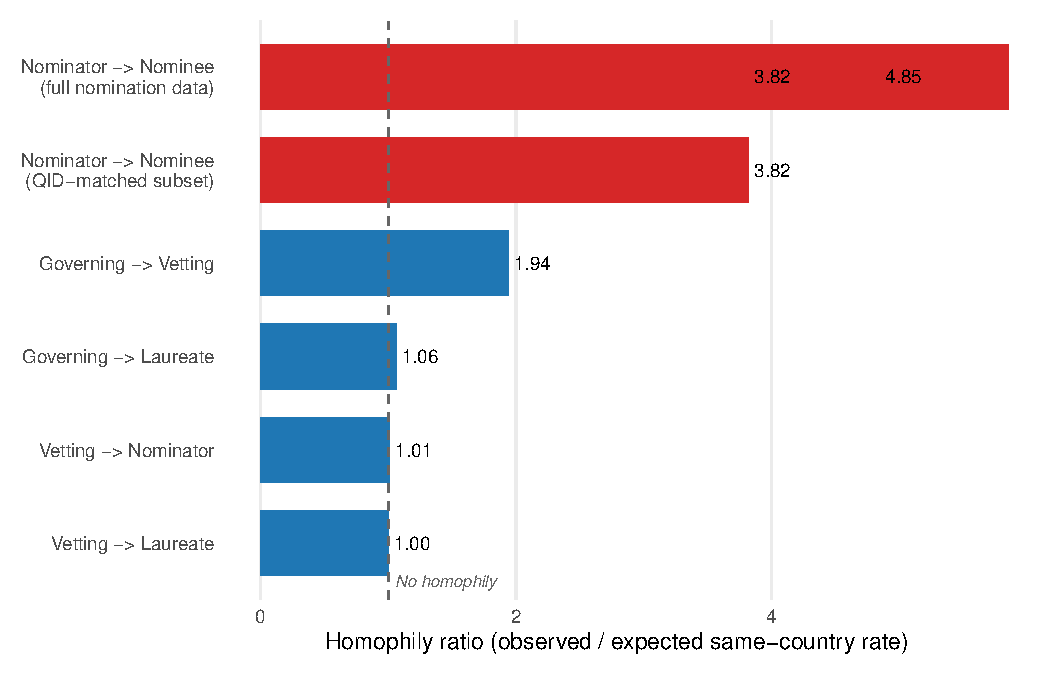
\includegraphics[width=\textwidth]{Figures/fig1_edge_type_homophily.pdf}
\caption{Country-level geographic homophily ratios by edge type. Red bars indicate nominator $\to$ nominee edges; blue bars indicate institutional edges. The dashed line at 1.0 marks the null expectation under random pairing. Homophily is concentrated in the nomination edge; institutional edges show ratios near 1.0.\label{fig:edge_homophily}}
\end{figure}

\subsection{Homophily Varies Across Disciplines}

Geographic homophily varies substantially across the five Nobel Prize categories, in a pattern consistent with the degree to which each discipline's knowledge networks are internationally integrated. Figure~\ref{fig:prize_homophily} presents homophily ratios at three geographic scales for each prize.

At the country level, the Nobel Prize in Literature exhibits the strongest homophily (ratio 8.58, $p < 0.001$), followed by Peace (5.26), Physiology/Medicine (5.16), Chemistry (3.55), and Physics (3.01). This ordering is interpretable: literature is bound to language, which correlates strongly with geography, while physics and chemistry deal in mathematical formalisms that are internationally legible regardless of the researcher's country of origin. The Peace Prize occupies a middle position, reflecting the mix of nationally prominent political figures and internationally recognized activists in its nominee pool.

Self-nomination rates by prize and subregion sharpen this picture. In Literature, Southern European nominators direct 92.7\% of their nominations to Southern European nominees, and Eastern European nominators direct 85.7\% to Eastern European nominees. In Physics, the same subregions self-nominate at rates of only 24.9\% and 41.3\%, respectively. Northern America self-nominates at 81.4\% in Physiology/Medicine and 76.8\% in Physics, but only 44.4\% in Literature, where American nominators look outward more than in the sciences.

\begin{figure}[t!]
\centering
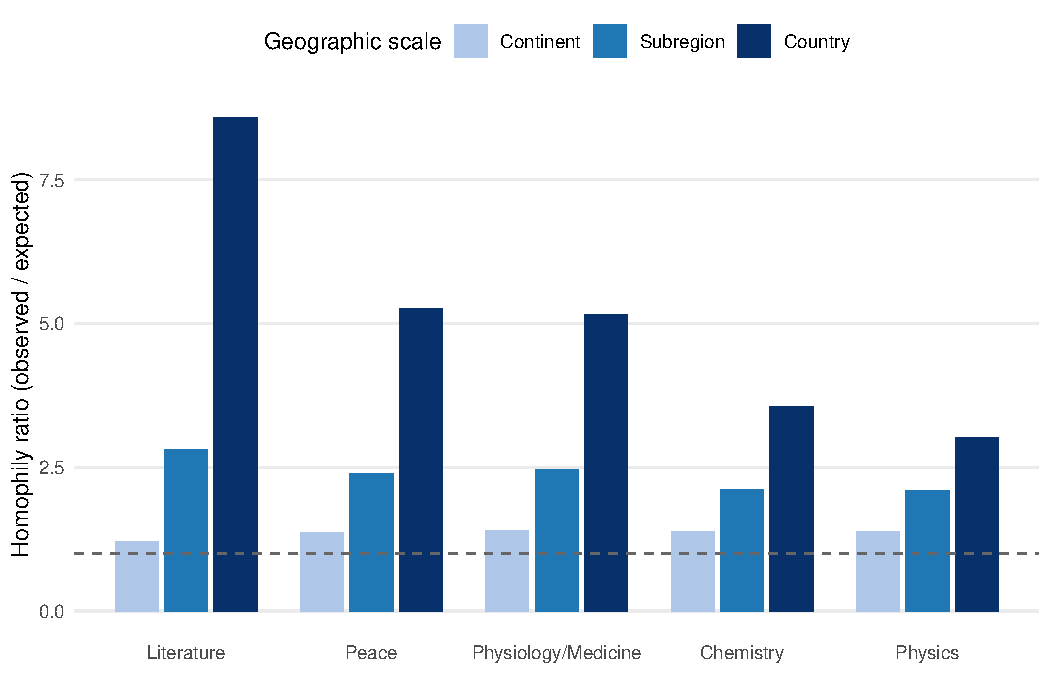
\includegraphics[width=\textwidth]{Figures/fig2_prize_homophily.pdf}
\caption{Nominator $\to$ nominee homophily ratios by Nobel Prize category at three geographic scales (continent, subregion, country). Homophily is strongest for Literature and weakest for Physics, consistent with the internationality of each discipline's knowledge networks.\label{fig:prize_homophily}}
\end{figure}

\subsection{The Globalization Paradox: Rising Relative Homophily}

The nominee pool has diversified substantially over the 20th century. The share of European nominees fell from 94.2\% in the 1900s to 55.7\% in the 1970s, and the effective number of continents represented among nominees rose from 1.28 to 2.52 over the same period (Figure~\ref{fig:temporal}, panel A; Table~\ref{tab:temporal_homophily}). Despite this diversification, the homophily ratio \emph{increased}, rising from 1.07 in the 1900s to a peak of 1.54 in the 1940s before stabilizing at 1.43--1.45 through the 1970s (Figure~\ref{fig:temporal}, panel B).

\begin{table}[ht]
\centering
\caption{Temporal trends in nominee pool diversity and nomination homophily. Homophily ratio $H = O/E$ measures continent-level geographic matching relative to random expectation, with 95\% CI. $r$ is Newman's assortativity. $O - E$ is the absolute excess same-continent rate in percentage points. $p$-values from 10{,}000 permutations; $p_{\text{adj}}$ is Bonferroni-adjusted across 49 formal tests.}
\label{tab:temporal_homophily}
\small
\begin{tabular}{lrrrrrrrrcc}
\toprule
Decade & $N$ & \% Eur. & Eff. cont. & Obs. & Exp. & $O - E$ & Ratio [95\% CI] & $r$ & $p$ & $p_{\text{adj}}$ \\
\midrule
1900s & 2,825 & 94.2 & 1.28 & 95.6\% & 89.0\% & 6.6 & 1.07 [1.00, 1.00] & 0.599 & $<$0.001 & 0.005 \\
1910s & 2,634 & 89.4 & 1.45 & 92.8\% & 82.6\% & 10.1 & 1.12 [0.99, 1.01] & 0.584 & $<$0.001 & 0.005 \\
1920s & 3,193 & 81.2 & 1.75 & 88.1\% & 72.5\% & 15.6 & 1.21 [0.99, 1.01] & 0.567 & $<$0.001 & 0.005 \\
1930s & 4,206 & 70.8 & 2.08 & 82.1\% & 59.6\% & 22.5 & 1.38 [0.98, 1.02] & 0.558 & $<$0.001 & 0.005 \\
1940s & 2,151 & 57.4 & 2.21 & 76.7\% & 49.7\% & 27.0 & 1.54 [0.96, 1.04] & 0.536 & $<$0.001 & 0.005 \\
1950s & 3,178 & 54.5 & 2.25 & 70.6\% & 48.7\% & 22.0 & 1.45 [0.97, 1.03] & 0.428 & $<$0.001 & 0.005 \\
1960s & 4,417 & 55.1 & 2.40 & 69.4\% & 48.2\% & 21.2 & 1.44 [0.97, 1.03] & 0.409 & $<$0.001 & 0.005 \\
1970s & 3,240 & 55.7 & 2.52 & 65.6\% & 45.7\% & 19.9 & 1.43 [0.97, 1.03] & 0.366 & $<$0.001 & 0.005 \\
\bottomrule
\end{tabular}
\end{table}


This pattern arises because the absolute same-continent nomination rate decreased (from 95.6\% to 65.6\%) but the expected rate under random pairing decreased faster (from 89.0\% to 45.7\%). In the early decades, the nominee pool was so overwhelmingly European that nearly any nomination would pair same-continent individuals by chance alone, leaving little room for detectable homophily. As the pool diversified, the expected same-continent rate fell, but nomination behavior did not diversify proportionally --- the gap between observed and expected widened. The 1940s peak likely reflects the geographic constraints of World War II, which restricted international scientific communication and may have further concentrated nominations within regions.

The implication is that the Nobel system has become more globally inclusive in absolute terms while becoming more geographically biased in relative terms. The same-continent preference was always present, but it became measurable only as the nominee pool heterogenized enough to provide a non-trivial null expectation.

\begin{figure}[t!]
\centering
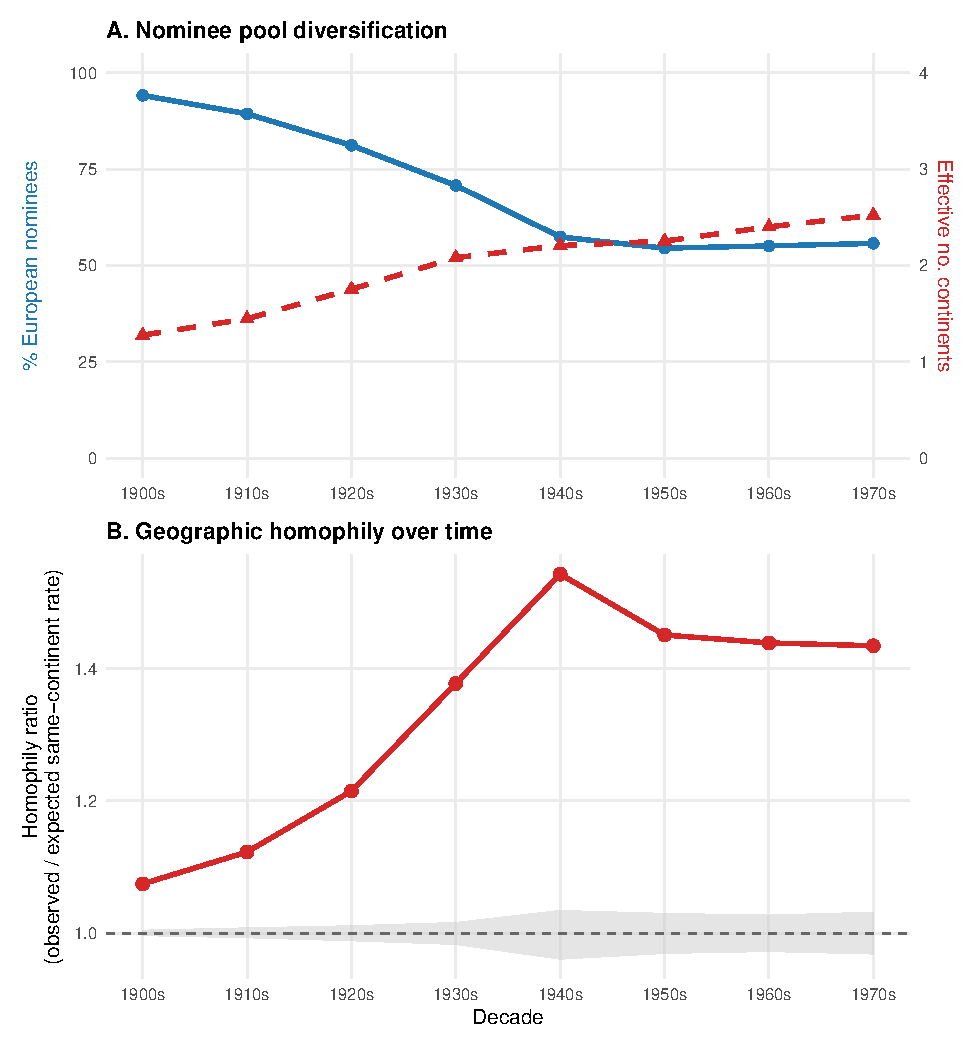
\includegraphics[width=\textwidth]{Figures/fig3_temporal_homophily.pdf}
\caption{The globalization paradox. (A) Diversification of the nominee pool: the share of European nominees (blue) declines while the effective number of continents (red, dashed) increases. (B) Continent-level homophily ratio over time, with the 95\% permutation reference interval in grey. The ratio rises from near 1 in the 1900s to approximately 1.5 in the 1940s, then plateaus, indicating that nomination behavior has not diversified proportionally to the nominee pool.\label{fig:temporal}}
\end{figure}

\section{Discussion}
\label{sec:discussion}

The central result of this study is that geographic homophily in the Nobel Prize network is overwhelmingly localized to a single decision point: the nominator's choice of whom to nominate. The institutional edges connecting governing bodies, vetting bodies, and laureates are geographically neutral. This decomposition has both methodological and substantive implications.

\subsection{Where Bias Enters}

The fact that institutional edges show no detectable homophily is not obvious \textit{a priori}. The governing and vetting bodies are nearly entirely Swedish, and one might reasonably expect that Swedish-led institutions would preferentially channel recognition toward Scandinavian or European scientists at every stage. Instead, the data show that the institutional machinery of the Nobel system operates without measurable geographic favoritism. The Nobel Committees invite a geographically diverse set of nominators (vetting body $\to$ nominator homophily ratio 1.01, $p = 0.070$), and the governing bodies select laureates without detectable geographic preference (ratio 1.01 at the continent level). The geographic sorting enters one step later, when those nominators --- who have been invited through a geographically neutral process --- choose whom to nominate.

This pattern is consistent with \citet{DumTep2025}, who find that same-country peer reviewers are approximately five percentage points more likely to recommend acceptance in scientific journals. Their work demonstrates that geographic homophily in evaluation is not an idiosyncrasy of any single institution but a systemic feature of how scientists assess one another. Our results extend this finding to the Nobel system and localize it more precisely: it is the discretionary judgment of individual evaluators, not institutional policy, that introduces geographic sorting.

\subsection{Mechanisms}

What drives nominators to favor geographically proximate nominees? At least three mechanisms are plausible. First, \emph{visibility}: scientists are more likely to be familiar with work produced in their own country, read by their own colleagues, and presented at their own conferences. This is a knowledge-access explanation. Second, \emph{epistemic affinity}: nominators may genuinely believe that work in their own tradition is of higher quality, not because of conscious partiality but because their evaluative frameworks were shaped by the same intellectual context. Third, \emph{strategic nationalism}: nominators may consciously or semiconsciously advocate for compatriots to enhance national scientific prestige. Our data cannot distinguish among these mechanisms, but the discipline gradient provides suggestive evidence. Literature, which is bound to language and national literary traditions, shows the strongest homophily (8.58$\times$ at the country level), while physics and chemistry, whose formalisms are internationally legible, show the weakest (3.01$\times$ and 3.55$\times$). This gradient is more consistent with the visibility and epistemic-affinity explanations than with strategic nationalism, which would not obviously vary across disciplines.

\subsection{Consequences for the Flow of Recognition}

The combination of geographic homophily and asymmetric pool composition generates systematic imbalances in the flow of recognition (Figure~\ref{fig:flow}). Northern America is the largest net importer of nominations, with a return ratio of 1.44 (6{,}802 nominations received vs.\ 4{,}714 sent). Northern Europe is the largest net exporter (return ratio 0.73, deficit of $-$1{,}860). Notably, the region that administers the Nobel system sends far more nominations outward than it receives.

\begin{figure}[t!]
\centering
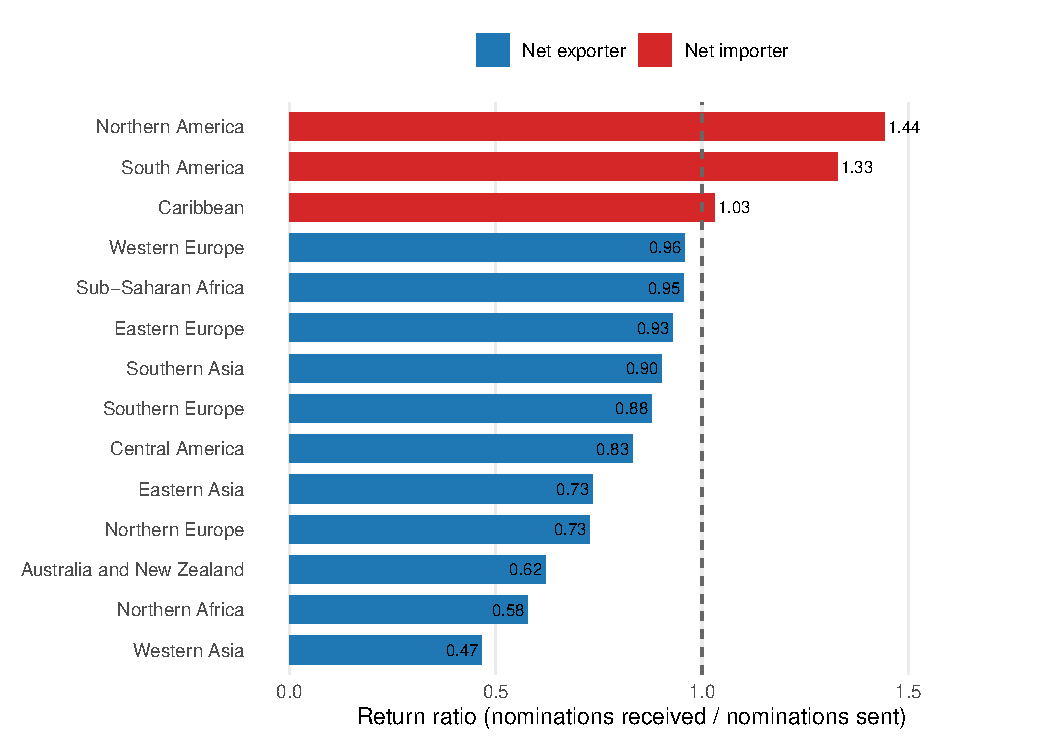
\includegraphics[width=\textwidth]{Figures/fig4_flow_asymmetry.pdf}
\caption{Return ratios (nominations received / nominations sent) by UN subregion. Red bars indicate net importers of recognition (ratio $> 1$); blue bars indicate net exporters. Northern America is the largest net importer; Northern Europe, which houses the Nobel Prize institutions, is the largest net exporter.\label{fig:flow}}
\end{figure}

These flows are a downstream consequence of the homophily documented in the preceding sections. When nominators preferentially nominate within their own geography, the result is a net transfer of recognition from regions overrepresented among nominators (Northern Europe) to regions overrepresented among nominees (Northern America). In the framework of \citet{Mer1968}, this constitutes a geographic dimension of the Matthew effect: regions that already concentrate scientific prestige receive a disproportionate share of nominations, which reinforces the very concentration that produced the imbalance.

\subsection{The Globalization Paradox and Its Implications}

The temporal finding --- that relative homophily has \emph{increased} even as the nominee pool has diversified --- has direct implications for policy. It suggests that simply expanding the geographic diversity of the nominee pool is insufficient to reduce geographic bias if nomination behavior does not change proportionally. The Nobel system has, by this measure, become more globally inclusive in absolute terms while becoming more geographically biased in relative terms. The same-continent preference was always present, but it became detectable only as the pool diversified enough to provide a non-trivial null expectation.

This pattern implies that the nomination stage is the critical intervention point. Structural reforms such as geographically stratified nomination quotas, explicit instructions to nominators to consider international candidates, or de-biasing training for invited nominators could, in principle, address the source of the homophily we document. Whether such reforms are desirable or feasible is a question of scientific governance that our data inform but do not resolve.

\subsection{Limitations}

Several limitations constrain our analysis. First, the nomination archive is subject to a 50-year secrecy rule, so our data extend only through the mid-1970s. We cannot determine whether the patterns we document have persisted, intensified, or diminished in subsequent decades. Second, our entity resolution matched only 27.3\% of nomination archive individuals to Wikidata QIDs (86.5\% of those with birth years). While the full nomination dataset preserves the topological structure of nominator--nominee relationships and provides per-nomination geographic fields at 94.7--97.7\% completeness, cross-layer analyses are limited to the matched subset. Third, we assign each individual a single geographic identity based on birth country, which does not capture migration, dual nationality, or the country of professional activity at the time of nomination. Fourth, our measure of homophily is relative to a null model of random pairing; the appropriate normative benchmark for ``how much homophily is too much'' is a question our statistical framework does not address.

\section{Conclusions}
\label{sec:conclusions}

We have constructed the first comprehensive multilayer network of the Nobel Prize selection process, spanning all five original prize categories from 1901 through the most recent year of publicly available nomination data. By decomposing geographic homophily across five edge types, three geographic scales, five disciplines, and eight decades, we identify the nomination stage as the singular point at which geographic sorting enters an otherwise geographically neutral institutional process. This homophily varies across disciplines in a pattern consistent with the internationality of each field's knowledge networks, and it has intensified in relative terms even as the nominee pool has diversified. These findings demonstrate that geographic bias in the world's most prestigious scientific recognition system is not an institutional policy but an emergent property of individual evaluation behavior --- and that diversifying the candidate pool, while necessary, is not sufficient to correct it.

\bibliographystyle{plainnat}
\bibliography{bibliography}

\section*{Acknowledgments}

We are grateful to Atilio Barreda, William Bork Rodriguez, Drew Lewis, Jessica Libertini, Roland Molontay, Christy Mullican, Marcel Nagy, Carlos Paniagua, and Nguyen Tran for their contributions during the early stages of this work. We also thank the Institute for Computational and Experimental Research in Mathematics (ICERM), where this project was begun as part of a program on Data Science and Social Justice.

\end{document}
